\documentclass{article}\usepackage[]{graphicx}\usepackage[]{color}

\usepackage{alltt}
\usepackage{float}
\usepackage{graphicx}
\usepackage{tabularx}
\usepackage{siunitx}
\usepackage{amssymb} % for math symbols
\usepackage{amsmath} % for aligning equations
\usepackage{textcomp}
\usepackage{booktabs}
\usepackage{mdframed}
\usepackage{natbib}
\usepackage{comment}
\usepackage{booktabs}
\usepackage[colorinlistoftodos]{todonotes} % to make comments on the margin
\usepackage[small]{caption}
\setlength{\captionmargin}{30pt}
\setlength{\abovecaptionskip}{0pt}
\setlength{\belowcaptionskip}{10pt}
\topmargin -1.5cm        
\oddsidemargin -0.04cm   
\evensidemargin -0.04cm
\textwidth 16.59cm
\textheight 21.94cm 
%\pagestyle{empty} %comment if want page numbers
\parskip 7.2pt
\renewcommand{\baselinestretch}{1.5}
\parindent 0pt
%\usepackage{lineno}
%\linenumbers

%% R Script

\title{Supplementary Material}

% alternative titles:
%% An expanded bayesian phylogenetic mixed model to unravel the phenology-phylogeny tangle. %% this sounds too methodsy

\begin{document}

\maketitle

\noindent Authors:\\
The Wolkovich Lab in 2019 \& collaborators $^{1,2,3,4}$ % Will Pearse, Jonathan Davies also
\vspace{2ex}\\
\emph{Author affiliations:}\\
$^{1}$Forest \& Conservation Sciences, Faculty of Forestry, University of British Columbia, 2424 Main Mall, Vancouver, BC V6T 1Z4;\\
$^{2}$Arnold Arboretum of Harvard University, 1300 Centre Street, Boston, Massachusetts, USA;\\
$^{3}$Organismic \& Evolutionary Biology, Harvard University, 26 Oxford Street, Cambridge, Massachusetts, USA;\\
$^{4}$Edificio Ciencias, Campus Universitario 28805 Alcalá de Henares, Madrid, Spain\\
 

\vspace{2ex}
$^*$Corresponding author: ignacio.moralesc@uah.es\\
\renewcommand{\thetable}{\arabic{table}}
\renewcommand{\thefigure}{\arabic{figure}}
\renewcommand{\labelitemi}{$-$}
\setkeys{Gin}{width=0.8\textwidth}

%%%%%%%%%%%%%%%%%%%%%%%%%%%%%%%%%%%%%%%%%%%%%%%
%%%%%%%%%%%%%%%%%%%%%%%%%%%%%%%%%%%%%%%%%%%%%%%
\clearpage

\section*{Extended methods}


\section*{Additional results}




%\bibliography{phylorefs}
%\bibliographystyle{amnat}

%%%%%%%%%%%%%%%%%%%%%%%%%%%%%%%
% Tables and Figures
%%%%%%%%%%%%%%%%%%%%%%%%%%%%%%%
\section*{Tables and Figures} 



%IMC 22mar - we should decide among one of the next two figures, instead of having separate figures per cues?
% EMW (28Mar2022): I vote for the first one, but both are great!
\begin{figure} [H]
  \begin{center}
  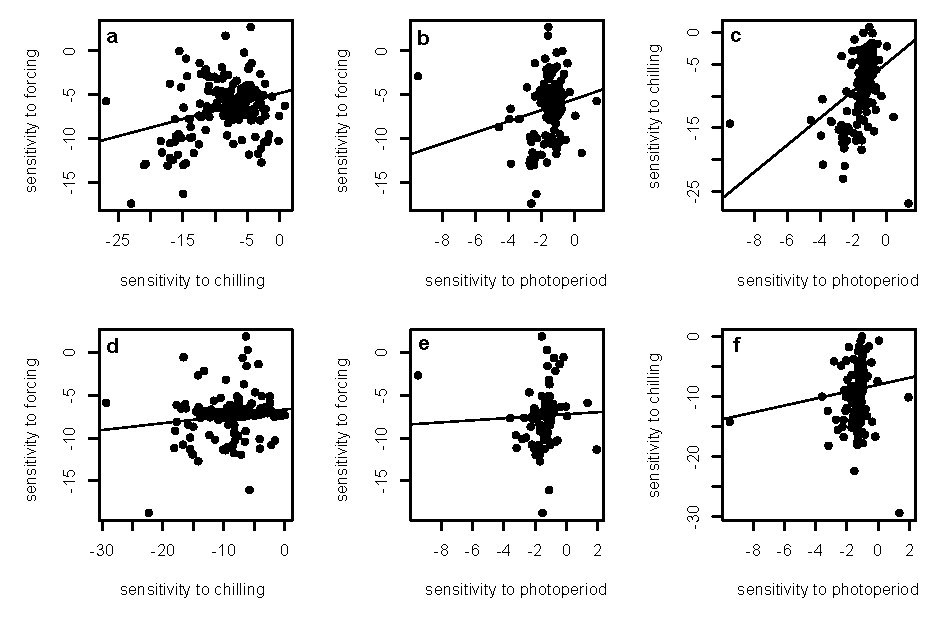
\includegraphics[width=16cm]{../../analyses/phylogeny/figures/FigSX_Sindromes_lamb_lamb0.pdf}
  \caption{Correlations among estimated sensitivities to the environmental cues comparing forcing vs. chilling (a,d), forcing vs. photoperiod (b,e) and chilling vs. photoperiod (c,f). Upper panels show correlations among estimated sensitivities by the phylogenetic model and panels  he color scale varies in each panel. Total tree depth is 81. My.}
  \label{fig:muplot_all}
  \end{center}
\end{figure}

\begin{figure} [H]
  \begin{center}
  \includegraphics[width=16cm]{../../analyses/phylogeny/figures/FigSXXX_comparison_eachsps_uncertainty.pdf}
  \caption{Phenological sensitivity to thee environmental cues, forcing (a), chilling (b) and photoperiod (c) measured in change in days to budburst per standardized unit (z-transformation) of the cues across 19 gymnosperm species. The same phylogenetic tree is shown in each panel, colored acording to an estimation of ancestral character states, being the states at the tips the model slopes of our hierarchical phylogenetic model. Note that the color scale varies in each panel. Total tree depth is 81. My.}
  \label{fig:muplot_allgymno}
  \end{center}
\end{figure}


\begin{figure} [H]
  \begin{center}
  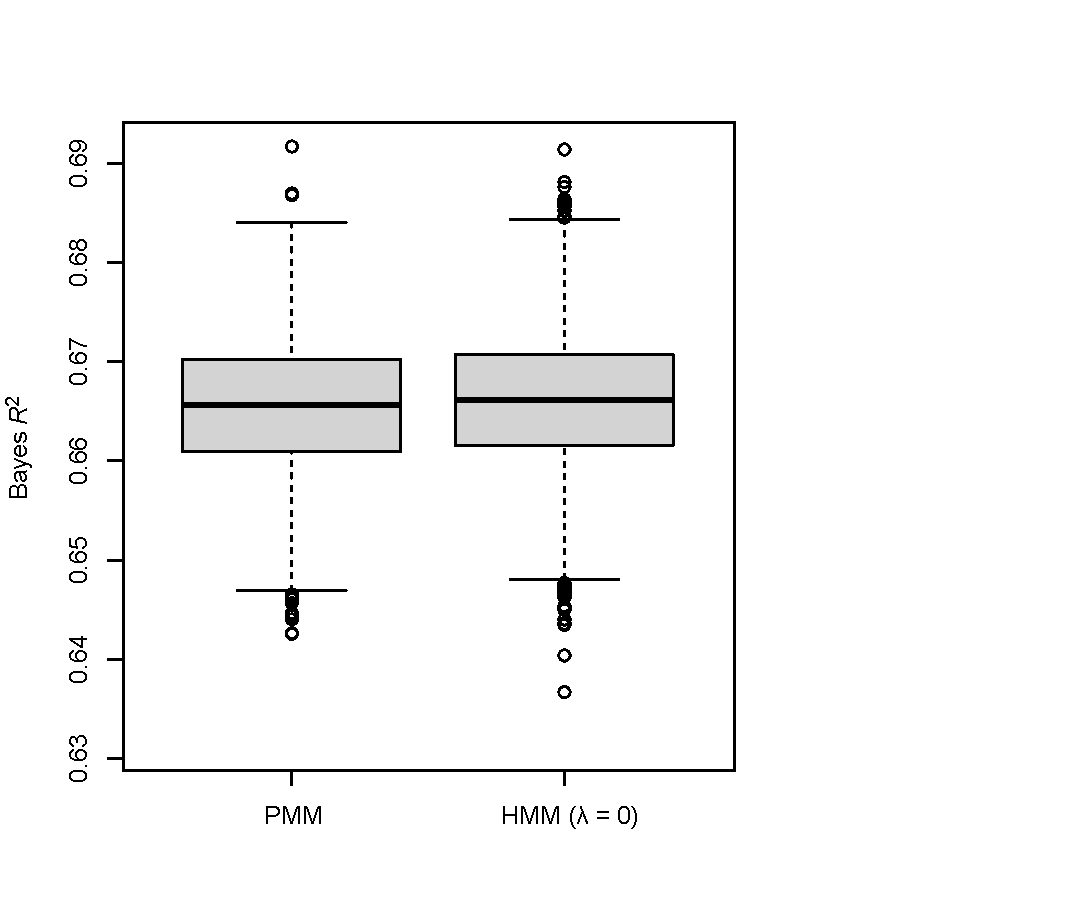
\includegraphics[width=14cm]{../../analyses/phylogeny/figures/Boxplot_bayesR2.pdf}
  \caption{Density plots for the posterior distribution of phylogenetic signal measured by lambda for each cue included as a predictor in the model for angiosperms: forcing (red), chilling (blue),  photoperiod (orange) and for the model intercept (grey). Panels correspond to angiosperms (a-d) and gymnosperms (e-h). Note that lambda estimations corresponding to  panels c-d and g-h as they are constrained to be either equal zero or equal 1.}
  \label{fig:phylosig_all}
  \end{center}
\end{figure}



\pagebreak
%\bibliographystyle{refs/bibstyles/amnat.bst}% 
%\bibliography{refs/phylorefs.bib}



\end{document}
